\documentclass{article}

\usepackage[left=2cm,right=2cm, top=2cm, bottom = 2cm]{geometry}
\usepackage{amsfonts}
%%%\usepackage{array}

\usepackage{amsmath}
\usepackage{xcolor}

\usepackage{tikz}
\usepackage{subfigure}

\pagestyle{empty}

\setlength{\tabcolsep}{15pt}
%%%\renewcommand{\arraystretch}{2.5}

%%%\makeatletter
%%%\newcommand{\thickhline}{%
%%%    \noalign {\ifnum 0=`}\fi \hrule height 2pt
%%%    \futurelet \reserved@a \@xhline
%%%}
%%%\newcolumntype{!}{@{\hskip\tabcolsep\vrule width 2pt\hskip\tabcolsep}}
%%%\makeatother

\newcommand{\deriv}[2]{\frac{\mathrm{d}#1}{\mathrm{d}#2}}
\newcommand{\diff}{\;\mathrm{d}}




\begin{document}

\title{Velocity and Integration}
\date{}

\maketitle
\thispagestyle{empty}

\Large

\textbf{\underline{Objective: To have an intuitive understanding of integration as}}

\textbf{\underline{it applies to velocity and areas under graphs.}}



\vspace{5mm}


{\bf Warm-up: Average and Instantaneous Speed:}

\vspace{5mm}

Usain Bolt runs for 10s, during which time he accelerates at a constant rate of $2\mathrm{ms^{-2}}$, starting from stationary.
\begin{enumerate}
	\item Write down an expression giving Bolt's velocity at time $t$, in terms of $a$ and $t$ (hint: acceleration is the derivative of velocity).
	\item Distance travelled is speed multiplied by time, but Bolt's speed is constantly changing, by the expression you found above. We will estimate the distance travelled in the 10s as follows:
		\begin{enumerate}
			\item Find Bolt's velocity after 5s; assuming he travels at this speed for the whole of the first 5s, find the distance he travels in these 5s.
			\item Find Bolt's velocity after 10s; assuming he travels at this speed for the whole of the last 5s (from 5s to 10s), find the distance he travels in these 5s.
			\item Add these two distances together for an estimate of the total distance travelled in the 10s of running.
		\end{enumerate}
		This graph illustrates the calculation:
		\begin{center}
		\begin{tikzpicture}[scale=0.5]
			\draw[->] (0,0) -- (10,0);
			\node[right] at (10,0) {$t$};
			\draw[->] (0,0) -- (0,10);
			\node[above] at (0,10) {$v$};
			\foreach \i in {0,2,...,10}{
				\node[below] at (\i,0) {$\i$};
			}
			\foreach \i in {0,4,...,20}{
				\node[left] at (0,0.5*\i) {$\i$};
			}
			
			\draw [thick,blue,domain=0:10,samples=10] plot (\x,{\x});
			\draw[dashed,red] (5,0) -- (5,5) -- (0,5);
			\draw[dashed,red] (10,0) -- (10,10) -- (5,10) -- (5,0);
		\end{tikzpicture}
		\end{center}
	\item Find a more accurate estimate of the distance travelled by dividing the time into 5 blocks of 2s each, and calculating the distance travelled in each block assuming that the speed for that block is constantly equal to the final speed at the end of the block. Draw a graph to illustrate this.
	\item Find the area underneath the velocity-time graph; explain why this must be equal to the distance travelled.
	\item By finding the area under the graph between time $0$ and time $t$, find an expression the distance Bolt runs in time $t$.
	\item Differentiate your expression for distance above to check you get your earlier expression for Bolt's velocity.
\end{enumerate}



\clearpage


{\bf Theory: Areas under Graphs:}

\vspace{5mm}

Velocity is the rate of change of distance with time; if velocity is constant, finding the distance travelled in a certain time is easy---you just multiply the velocity by the time. What if velocity is varying?

Suppose a particle moves with velocity function $v(t)=t^2$ in $\mathrm{ms^{-1}}$ and we want to find the distance travelled between time $t=0\mathrm{s}$ and time $t=5\mathrm{s}$. If the velocity were constant, we could find the distance simply by multiplying by the time, so we can estimate the total distance travelled by breaking our time interval up into 5 equal subintervals, say, and approximating the velocity by a constant in each subinterval.

\begin{center}
\begin{tikzpicture}[scale=0.5]
	\draw[->] (0,0) -- (10,0);
	\node[right] at (10,0) {$t$};
	\draw[->] (0,0) -- (0,12.5);
	\node[above] at (0,12.5) {$v$};
	\foreach \i in {0,...,5}{
		\node[below] at (2*\i,0) {$\i$};
	}
	\foreach \i in {0,4,...,24}{
		\node[left] at (0,0.5*\i) {$\i$};
	}
	
	\draw[blue,thick,domain=0:10,samples=100] plot (\x,{0.5*(0.5*\x)^2});
	
	\foreach \i in {1,...,5}{
		\draw[dashed,red] (2*\i,0) -- (2*\i,0.5*\i*\i) -- (2*\i-2,0.5*\i*\i) -- (2*\i-2,0.5*\i*\i-\i+0.5);
	}
	
\end{tikzpicture}
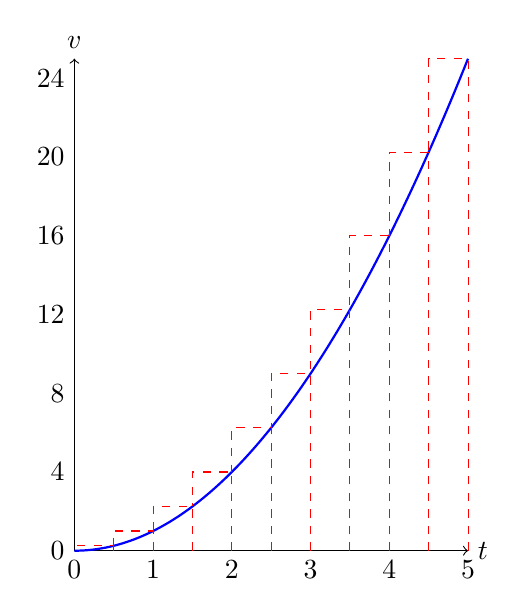
\begin{tikzpicture}[scale=0.5]
	\draw[->] (0,0) -- (10,0);
	\node[right] at (10,0) {$t$};
	\draw[->] (0,0) -- (0,12.5);
	\node[above] at (0,12.5) {$v$};
	\foreach \i in {0,...,5}{
		\node[below] at (2*\i,0) {$\i$};
	}
	\foreach \i in {0,4,...,24}{
		\node[left] at (0,0.5*\i) {$\i$};
	}
	
	\draw[blue,thick,domain=0:10,samples=100] plot (\x,{0.5*(0.5*\x)^2});
	
	\foreach \i in {1,...,10}{
		\draw[dashed,red] (\i,0) -- (\i,0.125*\i*\i) -- (\i-1,0.125*\i*\i) -- (\i-1,0.125*\i*\i-0.25*\i+0.125);
	}
	
\end{tikzpicture}
\end{center}

The red dashed rectangles in the left-hand graph have heights 1, 4, 9, 16, and 25 $\mathrm{ms}^{-1}$, respectively, and each has width 1s. Therefore the distance travelled in the 1s subintervals is roughly 1m, 4m, 9m, 16m, and 25m, respectively. Therefore the total distance travelled is roughly $1+4+9+16+25=55\mathrm{m}$.

We can see that the distance travelled in each 1s time interval is precisely the area of the rectangle. In order to get a more accurate estimate of the distance travelled, we would divide the time interval into a larger number of narrower subintervals, take the area of the rectangle over each subinterval, and add them up, as in the right-hand graph. It is clear that the greater the number and lesser the width of our subintervals, the more accurately we approximate the distance travelled, and the closer the rectangles approximate the total area. So in fact the distance travelled is precisely the area under the graph!

\clearpage













\textbf{Practice:}\bigskip


\begin{enumerate}
	\item Calculate the estimate of the distance travelled that comes by using 10 subintervals, as pictured in the right-hand graph above.
	\item Suppose we divide the time interval into $n$ equal subintervals. How long will each subinterval be (equivalently, how wide will each rectangle be)?
	\item If we take the estimated constant velocity (height of the rectangle) over each subinterval to be the value of the velocity at the right-hand endpoint of the subinterval, what will the height of the rectangle over the $k^\mathrm{th}$ subinterval be (in terms of $k$)?
	\item Hence show that using $n$ subintervals, our estimate for the area under the graph (total distance travelled) is
		\[\frac{125}{n^3}\sum_{k=1}^n k^2.\]
	\item Substitute the following formula
		\[\sum_{k=1}^n k^2=\frac{n}{6}(n+1)(2n+1)\]
		to find a formula for the approximate distance travelled. Substitute $n=5$ and $n=10$ into this formula and compare with the answer in the example above and your answer from question 1.
	\item By rearranging your formula, show that the distance travelled (area under the graph) is approximately
		\[\frac{125}{6}\left(1+\frac{1}{n}\right)\left(2+\frac{1}{n}\right).\]
	\item Now consider what happens as the number of subintervals is made arbitrarily large and their width infinitesimally small, by taking the limit of this expression as $n$ tends to infinity. Hence conclude the exact distance travelled by the particle between $t=0$ and $t=5$ (\textit{i.e.}, the exact area under the graph).
\end{enumerate}

\clearpage













\textbf{Theory: Integration:}\bigskip



In many problems, it is necessary to find the area under a graph. We have seen how the area underneath a velocity-time graph is the distance travelled; similarly, change in velocity is the area under an acceleration-time graph. If current is flowing onto a capacitor, the change in the total charge on the capacitor is the area under the current-time graph. If power is being dissipated in a resistor, the total energy dissipated is the area under the power-time graph. The variable on the horizontal axis need not be time---if a force is applied over a distance, the energy transferred is the area under the force-distance graph. There are countless other examples.

In each of these cases, we have a quantity (position, velocity, charge, energy, etc.) which changes with respect to some variable (often time, sometimes distance, etc.); for simplicity, we will assume change in time. If the rate-of-change of the quantity with respect to time were constant, the total change in the value of the quantity would simply be the constant rate-of-change multiplied by the time over which the change occurs---just like at a constant speed, the distance travelled is simply the speed times the time. When the rate-of-change of the quantity varies, we can break the time interval up into small subintervals and approximate the rate-of-change by a constant over that interval; we then add up the approximations over each subinterval to find an estimate for the total change in the quantity. This is the same as estimating the area under the graph of the rate-of-change against time.

By considering dividing up the time interval into a larger and larger number of narrower and narrower subintervals, we can construct more and more accurate estimates of the area under the graph (the change in the quantity whose rate-of-change is graphed). By taking a limit as the number of subintervals tends to infinity and hence their width tends to 0, we can find an exact value for the area under the graph. This process is called \textbf{integration}.\bigskip

Given a function $f(x)$, suppose we want to find the area under the graph of $f(x)$ between $x=a$ and $x=b$---\textit{i.e.}, we want to integrate $f(x)$ from $x=a$ to $x=b$. We can divide the interval from $a$ to $b$ into $n$ subintervals, each of length $\frac{b-a}{n}$. At the right-hand endpoint of the $k^\mathrm{th}$ subinterval, the value of the function is therefore
\[f\left(a+\frac{k(b-a)}{n}\right).\]

Multiplying this by the width of the subinterval and summing for $k$ from $1$ to $n$, we get an estimate of the total area:
\[\sum_{k=1}^nf\left(a+\frac{k(b-a)}{n}\right)\frac{b-a}{n}.\]

Now we let $n$ tend to infinity; since each subinterval has width $\frac{b-a}{n}$, the width of the subintervals tends to 0, but the number of them tends to infinity. The limit may or may not exist, but if it does, we call it the \textbf{integral of $f(x)$ from $a$ to $b$ with respect to $x$} and denote it:
\[\int_a^bf(x)\diff x=\lim_{n\to\infty}\sum_{k=1}^n f\left(a+\frac{k(b-a)}{n}\right)\frac{b-a}{n}.\]

If this limit exists, it should be precisely the area under the graph of $f(x)$ between $x=a$ and $x=b$. For any function you are ever likely to encounter, this will be true (with a caveat about signs to be dealt with next time); there are some very strange functions where a more subtle notion of integration called the Lebesgue integral is needed, but these are very unlikely to come up in an engineering context.

The notation for integration perhaps requires some explanation. The integral sign (the long, sinuous stroke) is a stretched out letter $S$, standing for ``sum,'' while the $\diff x$ is meant to stand for an infinitesimal change in $x$; the factor of $\frac{b-a}{n}$ in the sum (the width of each subinterval) can be thought of as a very small change in $x$, traditionally denoted $\delta x$, and then as we take the limit as $n$ tends to $\infty$, this $\delta x$ becomes arbitrarily small. The notation therefore stands for summing up values of $f(x)$ multiplied by small changes $dx$; it can often be useful to think of an integral as a sort of continuous analogue of a sum. If the function depends on a different variable, say $t$, we write that in the notation; so we have
\[\int_a^b f(t)\diff t,\]
for instance. The endpoints $a$ and $b$ of the interval we're integrating over are sometimes called the \textbf{limits of the integral} (no relation to limits as a variable tends to a number!).\bigskip



We argued in the discussion on the last page that if we take the area underneath the graph of the rate-of-change of a quantity, we should get the total change in the quantity; this is a profound insight known as the \textbf{Fundamental Theorem of Calculus}, which is undoubtedly one of the most important mathematical results ever discovered. We shall study this Fundamental Theorem next time.






\clearpage


{\bf Key Points to Remember:}

\vspace{5mm}

\begin{enumerate}
	\item The area under a graph over an interval on the $x$-axis can be estimated by dividing the interval up into a number of small subintervals, taking the area of the rectangle over each subinterval whose height is the value of the function at one point in the interval (say the right-hand endpoint), and adding up the areas of these rectangles. The more subintervals we take (and the smaller each subinterval is), the more accurate the estimate will be.
	\item Taking the limit of the above process as the number of subintervals tends to infinity and their width tends to 0, we obtain the exact value of the area under the graph, called the \textbf{integral}:
		\[\int_a^b f(x)\diff x=\lim_{n\to \infty}\sum_{k=1}^nf\left(a+\frac{k(b-a)}{n}\right)\frac{b-a}{n}.\]
	\item If the function we are integrating is the rate-of-change (derivative) of a quantity, we expect the area under the graph (the integral) to be the total change in that quantity between time $a$ and time $b$. We shall explore this more next time.
\end{enumerate}









\end{document}